\begin{figure}[htbp]
\section*{ACBD6}
\centering
\begin{subfigure}[b]{0.95\textwidth}
\centering
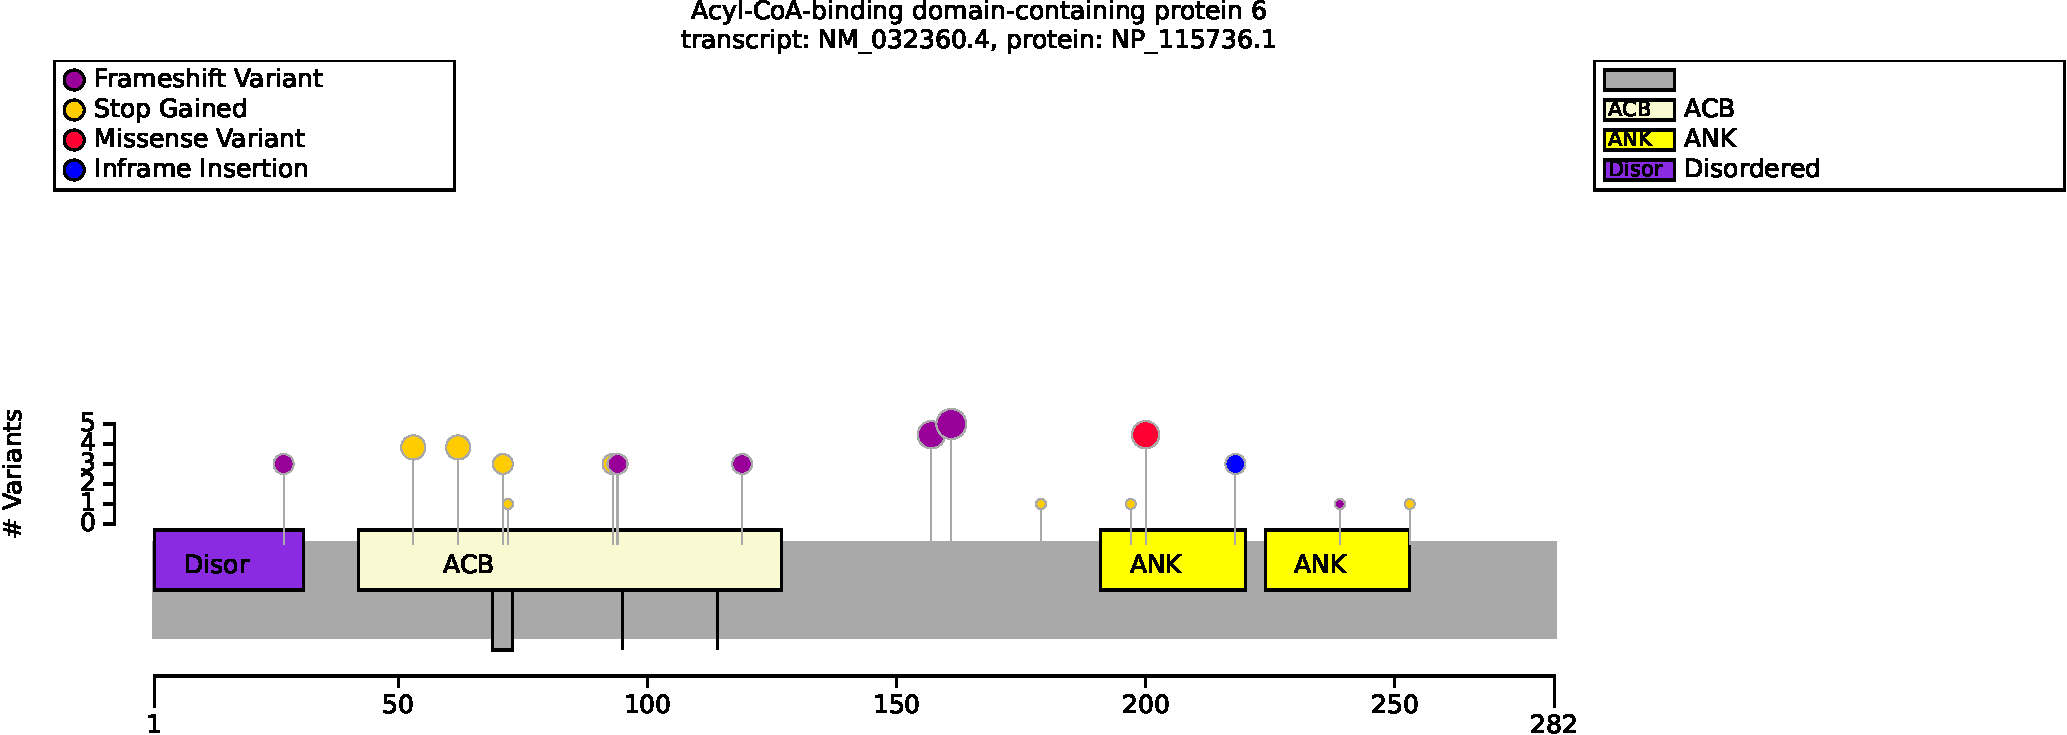
\includegraphics[width=\textwidth]{ img/ACBD6_protein_diagram.pdf} 
\captionsetup{justification=raggedright,singlelinecheck=false}
\caption{Distribution of variants in ACBD6}
\end{subfigure}

\vspace{2em}

\begin{subfigure}[b]{0.95\textwidth}
\centering
\resizebox{\textwidth}{!}{
\begin{tabular}{llllrr}
\toprule
Genotype (A) & Genotype (B) & total tests performed & significant results\\
\midrule
missense/missense OR missense/other & other/other & 99 & 0\\
\bottomrule
\end{tabular}
}
\captionsetup{justification=raggedright,singlelinecheck=false}
\caption{         Fisher Exact Test performed to compare HPO annotation frequency with respect to missense/missense OR missense/other and other/other. }
\end{subfigure}

\vspace{2em}

\begin{subfigure}[b]{0.95\textwidth}
\centering
\resizebox{\textwidth}{!}{
\begin{tabular}{llllrr}
\toprule
Genotype (A) & Genotype (B) & total tests performed & significant results\\
\midrule
ACB/ACB OR ACB/other & other/other & 99 & 0\\
\bottomrule
\end{tabular}
}
\captionsetup{justification=raggedright,singlelinecheck=false}
\caption{Fisher Exact Test performed to compare HPO annotation frequency with respect to ACB/ACB OR ACB/other and other/other. }
\end{subfigure}

\vspace{2em}

\begin{subfigure}[b]{0.95\textwidth}
\centering
\resizebox{\textwidth}{!}{
\begin{tabular}{llllrr}
\toprule
Genotype (A) & Genotype (B) & total tests performed & significant results\\
\midrule
FEMALE & MALE & 99 & 0\\
\bottomrule
\end{tabular}
}
\captionsetup{justification=raggedright,singlelinecheck=false}
\caption{Fisher Exact Test performed to compare HPO annotation frequency with respect to FEMALE and MALE.}
\end{subfigure}

\vspace{2em}

\caption{The cohort comprised 45 individuals (22 females, 23 males). A total of 79 HPO terms were used to annotate the cohort. Disease diagnosis: Neurodevelopmental disorder with progressive movement abnormalities (OMIM:620785). No statistically significant results identified. A total of 20 unique variant alleles were found in \textit{ACBD6} (transcript: \texttt{NM\_032360.4}, protein id: \texttt{NP\_115736.1}).}
\end{figure}
